\begin{name}
	{\tenchude}
	{\tendethi}
	{ĐỀ ÔN TẬP SỐ 2}
	{\thoigian}
\end{name}
	\setcounter{ex}{0}\setcounter{bt}{0}
	\Opensolutionfile{ans}[ans/ans-2-GHK1-32-NguyenThaiBinh-QuangNam-21]
\begin{ex}%[GHK1, THPT Nguyễn Thái Bình, Quảng Nam, 2021]%[Kiều Ngân, 12EX3-2021]%[2D1B2-3]
	Tìm tất cả các giá trị của $m$ để hàm số $y=\dfrac{1}{3}x^3-(m-1)x^2+(m^2-3m+2)x+5$ đạt cực đại tại $x=0$.
	\choice
	{\True $m=2$}
	{$m=-2$, $m=-1$}
	{$m=-1$}
	{$m=2$, $m=1$}
	\loigiai{
		Tập xác định $\mathscr{D}=\mathbb{R}$.\\
		Ta có $y'=x^2-2(m-1)x+m^2-3m+2$.\\
		Hàm số đạt cực đại tại $x=0$ $\Rightarrow y'(0)=0\Leftrightarrow m^2-3m+2=0 \Leftrightarrow \hoac{&m=1\\&m=2.}$\\
		Thử lại:
		\begin{itemize}
			\item $m=1$, ta có $y'=x^2$ và $y'=0\Leftrightarrow x=0$.
			\begin{center}
				
\begin{tikzpicture}[>=stealth,line join=round,line cap=round,scale=1]
				\tkzTabInit[lgt=1,espcl=2.5,deltacl=0.5]
				{$x$/0.6,$y'$/0.6,$y$/2}
				{$-\infty$,$0$,$+\infty$}
				\tkzTabLine{,+,$0$,+}
				\tkzTabVar{-/$-\infty$,R,+/$+\infty$}
				\end{tikzpicture}
			\end{center}
				Dựa vào bảng biến thiên ta thấy hàm số không đạt cực trị tại $x=0$. Do đó loại $m=1$.
			\item $m=2$, ta có $y'=x^2-2x$ và $y''=2x-2$ nên $y''(0)=-2<0$. Suy ra hàm số đạt cực đại tại $x=0$. Do đó nhận $m=2$.
		\end{itemize}
		Vậy $m=2$ thỏa yêu cầu đề bài.
	}
\end{ex}

\begin{ex}%[GHK1, THPT Nguyễn Thái Bình, Quảng Nam, 2021]%[Kiều Ngân, 12EX3-2021]%[2H1Y3-2]
	Cho khối lăng trụ có diện tích đáy bằng $3a^2$ và chiều cao bằng $4a$. Thể tích của khối lăng trụ đã cho bằng
	\choice
	{$4a^3$}
	{$36a^3$}
	{$48a^3$}
	{\True $12a^3$}
	\loigiai{
		Thể tích khối lăng trụ là $V=Sh=3a^2\cdot 4a=12a^3$.
	}
\end{ex}

\begin{ex}%[GHK1, THPT Nguyễn Thái Bình, Quảng Nam, 2021]%[Kiều Ngân, 12EX3-2021]%[2D1Y3-1]
	Giá trị nhỏ nhất của hàm số $f(x)=x^3-30x$ trên đoạn $[2;19]$ bằng
	\choice
	{$-63$}
	{$20\sqrt{10}$}
	{\True $-20\sqrt{10}$}
	{$-52$}
	\loigiai{
		Hàm số xác định và liên tục trên đoạn $[2;19]$.\\
		Ta có $y'=3x^2-30$ và $y'=0\Leftrightarrow \hoac{&x=\sqrt{10}\in [2;19]\\&x=-\sqrt{10}\notin [2;19].}$\\
		Tính $f(2)=-52$, $f(19)=$, $f(\sqrt{10})=-20\sqrt{10}$.\\
		Vậy $\min\limits_{[2;19]}f(x)=f(\sqrt{10})=-20\sqrt{10}$.
	}
\end{ex}

\begin{ex}%[GHK1, THPT Nguyễn Thái Bình, Quảng Nam, 2021]%[Kiều Ngân, 12EX3-2021]%[2D1Y1-1]
	Hàm số $y=-x^3+3x^2$ đồng biến trên khoảng nào dưới đây?
	\choice
	{$(0;4)$}
	{$(-\infty;0)$}
	{\True $(0;2)$}
	{$(2;+\infty)$}
	\loigiai{
		Tập xác định $\mathscr{D}=\mathbb{R}$.\\
		Ta có $y'=-3x^2+6x$ và $y'=0\Leftrightarrow \hoac{&x=0\\&x=2.}$\\
		Bảng biến thiên
		\begin{center}
			
\begin{tikzpicture}[>=stealth,line join=round,line cap=round,scale=1]
			\tkzTabInit[lgt=1,espcl=2.5,deltacl=0.5]
			{$x$/0.6,$y'$/0.6,$y$/2}
			{$-\infty$,$0$,$2$,$+\infty$}
			\tkzTabLine{,-,$0$,+,$0$,-,}
			\tkzTabVar{+/$+\infty$,-/$0$,+/$4$,-/$-\infty$}
			\end{tikzpicture}
		\end{center}
		Vậy hàm số đồng biến trên khoảng $(0;2)$.
	}
\end{ex}

\begin{ex}%[GHK1, THPT Nguyễn Thái Bình, Quảng Nam, 2021]%[Kiều Ngân, 12EX3-2021]%[2D1Y5-4]
	Số giao điểm của đồ thị hàm số $y=x^3+x^2$ và đồ thị hàm số $y=x^2+5x$ là
	\choice
	{$1$}
	{$2$}
	{$0$}
	{\True $3$}
	\loigiai{
		Phương trình hoành độ giao điểm của đồ thị hàm số $y=x^3+x^2$ và đồ thị hàm số $y=x^2+5x$ là
		$$x^3+x^2=x^2+5x\Leftrightarrow x^3-5x=0 \Leftrightarrow \hoac{&x=0\\&x=\pm \sqrt{5}.}$$
		Vậy có $3$ giao điểm giữa đồ thị hàm số $y=x^3+x^2$ và đồ thị hàm số $y=x^2+5x$.
	}
\end{ex}

\begin{ex}%[GHK1, THPT Nguyễn Thái Bình, Quảng Nam, 2021]%[Kiều Ngân, 12EX3-2021]%[2H1Y3-2]
	Cho khối hộp hình chữ nhật có ba kích thước $2$, $4$, $6$. Thể tích của khối hộp đã cho bằng
	\choice
	{$12$}
	{\True $48$}
	{$8$}
	{$16$}
	\loigiai{
		Thể tích của khối hộp chữ nhật là $2\cdot 4\cdot 6=48$.
	}
\end{ex}

\begin{ex}%[GHK1, THPT Nguyễn Thái Bình, Quảng Nam, 2021]%[Kiều Ngân, 12EX3-2021]%[2D1Y2-2]
	Cho hàm số $y=f(x)$ có bảng biến thiên như sau
	\begin{center}
		
\begin{tikzpicture}[>=stealth]
		\tkzTabInit[nocadre=false,lgt=1.2,espcl=2.5,deltacl=0.5]
		{$x$/.6 ,$f'(x)$/.6,$f(x)$/2}
		{$-\infty$ , $-1$ , $2$ , $+\infty$}
		\tkzTabLine{ , - , $0$ , + , $0$ , - , }
		\tkzTabVar{+/$+\infty$ , -/$-3$ , +/$1$ , -/$-\infty$}
		\end{tikzpicture}
	\end{center}
	Hàm số đã cho đạt cực tiểu tại
	\choice
	{$x=-3$}
	{$x=2$}
	{\True $x=-1$}
	{$x=1$}
	\loigiai{
		Dựa vào bảng biến thiên ta thấy hàm số đã cho đạt cực tiểu tại $x=-1$.	
	}
\end{ex}

\begin{ex}%[GHK1, THPT Nguyễn Thái Bình, Quảng Nam, 2021]%[Kiều Ngân, 12EX3-2021]%[2H1Y1-2]
	Cho một hình đa diện. Khẳng định nào sau đây là \textbf{sai}?
	\choice
	{Mỗi cạnh của một khối đa diện là cạnh chung của đúng hai mặt}
	{Mỗi mặt có ít nhất ba cạnh}
	{Mỗi đỉnh là đỉnh chung của ít nhất ba mặt}
	{\True Hai mặt bất kì luôn có ít nhất một điểm chung}
	\loigiai{
		Hai mặt bất kì của hình đa diện có thể có điểm chung hoặc không có điểm chung.
	}
\end{ex}

\begin{ex}%[GHK1, THPT Nguyễn Thái Bình, Quảng Nam, 2021]%[Kiều Ngân, 12EX3-2021]%[2D1Y2-2]
	Cho hàm số $y=f(x)$ liên tục trên $\mathbb{R}$ và có bảng xét dấu của $f'(x)$ như sau
	\begin{center}
		
\begin{tikzpicture}[>=stealth]
		\tkzTabInit[nocadre=false,lgt=1.2,espcl=2.5,deltacl=0.5]
		{$x$/.6 ,$f'(x)$/.6}
		{$-\infty$, $-1$, $2$, $3$, $+\infty$}
		\tkzTabLine{ ,-,d,+,$0$,+,$0$,-, }
		\end{tikzpicture}
	\end{center}
	Số điểm cực trị của hàm số $f(x)$ là
	\choice
	{$0$}
	{$3$}
	{\True $2$}
	{$1$}
	\loigiai{
		Dựa vào bảng xét dấu $f'(x)$ ta suy ra bảng biến thiên có thể có của hàm số $f(x)$
		\begin{center}
			
\begin{tikzpicture}[>=stealth]
			\tkzTabInit[nocadre=false,lgt=1.2,espcl=2.5,deltacl=0.5]
			{$x$/.6 ,$f'(x)$/.6,$f(x)$/2}
			{$-\infty$, $-1$, $2$, $3$, $+\infty$}
			\tkzTabLine{ ,-,d,+,$0$,+,$0$,-, }
			\tkzTabVar{+/$+\infty$,-/$f(-1)$,R,+/$f(3)$,-/$-\infty$}
			\end{tikzpicture}
		\end{center}
		Vậy hàm số $f(x)$ có hai điểm cực trị.
	}
\end{ex}

\begin{ex}%[GHK1, THPT Nguyễn Thái Bình, Quảng Nam, 2021]%[Kiều Ngân, 12EX3-2021]%[2D1K2-2]
	\immini{
		Cho hàm số $f(x)=ax^3+bx^2+cx+d$ có đồ thị như hình vẽ bên. Số điểm cực trị của hàm số $y=f(-2x^2+4x)$ là
		\choice
		{$4$}
		{$2$}
		{\True $5$}
		{$3$}
	}{
		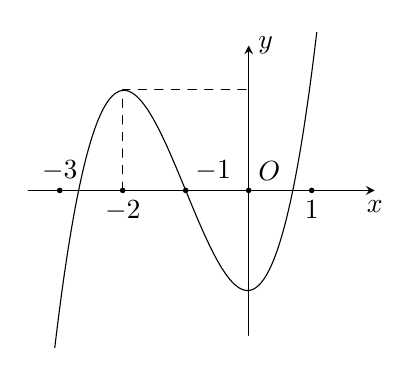
\begin{tikzpicture}[>=stealth,line join=round,line cap=round,font=\normalsize,scale=0.8]
		\draw[->] (-3.5,0)--(0,0) node[above right]{$O$}--(2,0) node[below]{$x$};
		\draw[->] (0,-2.3)--(0,2.3) node[right]{$y$};
		\clip (-3.5,-2.5) rectangle (2,2.5);
		\draw [domain=-3.1:1.1, samples=300] %
		plot (\x, {0.84*(\x+1)*(\x+2.7)*(\x-0.7)});
		\foreach \i in {-3,-2,-1,0,1}
		\draw[fill=black] (\i,0) circle (1pt);
		\foreach \i in {-2,1}
		\node[below] at (\i,0) {$\i$};
		\node[above right] at (-1,0) {$-1$};
		\node[above] at (-3,0) {$-3$};
		\draw[dashed] (-2,0)--(-2,1.6)--(0,1.6);
		\end{tikzpicture}
	}
	\loigiai{
		Đặt $g(x)=f(-2x^2+4x)$.\\
		Ta có $g'(x)=(-2x^2+4x)'f'(-2x^2+4x)=(-4x+4)f'(-2x^2+4x)$.\\ Khi đó
		$$g'(x)=0\Leftrightarrow \hoac{&x=1\\&-2x^2+4x=-2\\&-2x^2+4x=0}\Leftrightarrow \hoac{&x=1\\&x=1-\sqrt{2}\\&x=1+\sqrt{2}\\&x=0\\&x=2.}$$
		Các nghiệm của phương trình $g'(x)=0$ đều là nghiệm đơn nên hàm số $y=f(-2x^2+4x)$ có $5$ điểm cực trị. 
	}
\end{ex}

\begin{ex}%[GHK1, THPT Nguyễn Thái Bình, Quảng Nam, 2021]%[Kiều Ngân, 12EX3-2021]%[2D1B4-1]
	Tổng số tiệm cận đứng và tiệm cận ngang của đồ thị hàm số $y=\dfrac{5x^2-4x-1}{x^2-1}$ là
		\choice
		{$0$}
		{$3$}
		{$1$}
		{\True $2$}
	\loigiai{
		Tập xác định $\mathscr{D}=\mathbb{R}\setminus\{-1;1\}$.\\
		Ta có
		\begin{itemize}
			\item $\lim\limits_{x\to \pm \infty}y=5$. Suy ra $y=5$ là đường tiệm cận ngang của đồ thị hàm số.
			\item $\lim\limits_{x\to 1}y=\lim\limits_{x\to 1}\dfrac{(x-1)(5x+1)}{(x-1)(x+1)}=\lim\limits_{x\to 1}\dfrac{5x+1}{x+1}=3$. Suy ra $x=1$ không là đường tiệm cận đứng của đồ thị hàm số.
			\item $\lim\limits_{x\to (-1)^-}y=+\infty$. Suy ra $x=-1$ là đường tiệm cận đứng của đồ thị hàm số.
		\end{itemize}
		Vậy tổng số đường tiệm cận đứng và ngang của đồ thị hàm số là $2$.
	}
\end{ex}

\begin{ex}%[GHK1, THPT Nguyễn Thái Bình, Quảng Nam, 2021]%[Kiều Ngân, 12EX3-2021]%[2D1B3-1]
	Giá trị lớn nhất của hàm số $y=\dfrac{x-2}{x-3}$ trên $[0;2]$ bằng
	\choice
	{$-5$}
	{\True $\dfrac{2}{3}$}
	{$\dfrac{1}{3}$}
	{$0$}
	\loigiai{
		Hàm số xác định và liên tục trên đoạn $[0;2]$.\\
		Ta có $y'=\dfrac{-1}{(x-3)^2}<0,\,\forall x\ne 3$.	Do đó hàm số nghịch biến trên đoạn $[0;2]$.\\
		Vậy $\max\limits_{[0;2]}y=y(0)=\dfrac{2}{3}$.
	}
\end{ex}

\begin{ex}%[GHK1, THPT Nguyễn Thái Bình, Quảng Nam, 2021]%[Kiều Ngân, 12EX3-2021]%[1H3B5-3]
	Cho hình chóp $S.ABCD$ có đáy $ABCD$ là hình thoi cạnh $a$ và $\widehat{BAD}=60^\circ$. Cạnh bên $SA$ vuông góc với mặt phẳng đáy, góc giữa $SC$ và mặt đáy bằng $60^\circ$. Khoảng cách từ $C$ đến mặt phẳng $(SBD)$ là
	\choice
	{\True $\dfrac{3a}{\sqrt{13}}$}
	{$\dfrac{a}{\sqrt{13}}$}
	{$\dfrac{9a}{\sqrt{13}}$}
	{$\dfrac{a\sqrt{3}}{7}$}
	\loigiai{
		\immini{
			Ta có $ABCD$ là hình thoi cạnh $a$ và $\widehat{BAD}=60^\circ$ nên tam giác $ABD$, $CBD$ là hai tam giác đều cạnh $a$.\\
			Vì $SA\perp (ABCD)$ nên $AC$ là hình chiếu của $SC$ lên mặt $(ABCD)$. Suy ra góc giữa $SC$ và $(ABCD)$ là $\widehat{SCA}=60^\circ$.\\
			Gọi $O$ là tâm hình thoi $ABCD$.\\
			Kẻ $AH\perp SO$ tại $H$.\\
			Ta có $\heva{&BD\perp AC\\&BD\perp SA}\Rightarrow BD\perp (SAC) \Rightarrow BD\perp AH$.
		}{
			\begin{tikzpicture}[>=stealth,line join=round,line cap=round,font=\normalsize,scale=0.9]
			\coordinate (A) at (0,0);
			\coordinate (D) at (4,0);
			\coordinate (B) at (-2,-1);
			\coordinate (C) at ($(B)+(D)-(A)$);
			\coordinate (S) at ($(A)+(0,3.5)$);
			\coordinate (O) at ($(A)!0.5!(C)$);
			\coordinate (H) at ($(S)!0.6!(O)$);
			\draw (S)--(B)--(C)--(S)--(D)--(C);
			\draw [dashed] (O)--(S)--(A)--(C) (B)--(D)--(A)--(B) (A)--(H);
			\foreach \i in {A,B,C,D,S,O,H}
			\draw[fill=black] (\i) circle(1pt);
			\node[below] at (B) {$B$};
			\node[below] at (C) {$C$};
			\node[above left] at (A) {$A$};
			\node[right] at (D) {$D$};
			\node[below] at (O) {$O$};
			\node[above] at (S) {$S$};
			\node at ($(H)+(0.2,0)$) {$H$};
			\tkzMarkRightAngles (S,A,O S,H,A A,O,B)
			\end{tikzpicture}
		}
		\noindent
		Do dó $\heva{&AH\perp BD\\&AH\perp SO}\Rightarrow AH\perp (SBD)$
		$\Rightarrow \mathrm{d}(C,(SBD))=\mathrm{d}(A,(SBD))=AH$.\\
		Ta có $AO=\dfrac{a\sqrt{3}}{2}\Rightarrow AC=2AO=a\sqrt{3}$; $SA=AC\cdot \tan \widehat{SCA}=a\sqrt{3}\cdot \sqrt{3}=3a$.\\
		Khi đó $\dfrac{1}{AH^2}=\dfrac{1}{SA^2}+\dfrac{1}{AO^2}=\dfrac{1}{9a^2}+\dfrac{4}{3a^2}=\dfrac{13}{9a^2}\Rightarrow AH=\dfrac{3a}{\sqrt{13}}$.
	}
\end{ex}

\begin{ex}%[GHK1, THPT Nguyễn Thái Bình, Quảng Nam, 2021]%[Kiều Ngân, 12EX3-2021]%[2D1B3-1]
	\immini{
		Cho hàm số $y=f(x)$ liên tục trên đoạn $[-1;3]$ và có đồ thị như hình vẽ. Gọi $M$ và $m$ lần lượt là giá trị lớn nhất, giá trị nhỏ nhất của hàm số đã cho trên đoạn $[-1;3]$. Giá trị của $M-m$ bằng
		\choice
		{$1$}
		{$4$}
		{\True $5$}
		{$0$}
	}{
		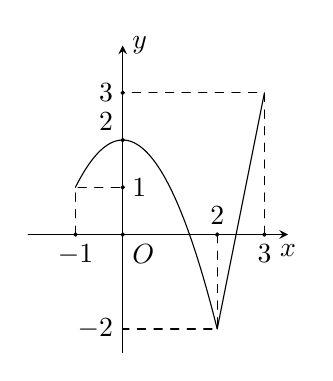
\begin{tikzpicture}[>=stealth,line join=round,line cap=round,font=\normalsize,scale=0.6]
		\draw[->] (-2,0)--(0,0) node[below right]{$O$}--(3.5,0) node[below]{$x$};
		\draw[->] (0,-2.5)--(0,4) node[right]{$y$};
		\clip (-2,-2.5) rectangle (3.5,4);
		\draw [domain=-1:2, samples=300] %
		plot (\x, {-(\x)^2+2});
		\draw (2,-2)--(3,3);
		\foreach \i in {-1,0,2,3}
		\draw[fill=black] (\i,0) circle (1pt);
		\foreach \j in {1,2,3}
		\draw[fill=black] (0,\j) circle (1pt);
		\node[below] at (-1,0) {$-1$};
		\node[above] at (2,0) {$2$};
		\node[below] at (3,0) {$3$};
		\node[right] at (0,1) {$1$};
		\node[left] at (0,-2) {$-2$};
		\node[above left] at (0,2) {$2$};
		\node[left] at (0,3) {$3$};
		\draw[dashed] (-1,0)--(-1,1)--(0,1) (2,0)--(2,-2)--(0,-2) (3,0)--(3,3)--(0,3);
		\end{tikzpicture}
	}
	\loigiai{
		Dựa vào đồ thị hàm số ta thấy
		\begin{itemize}
			\item $\max\limits_{[-1;3]}y=y(3)=3$ $\Rightarrow M=3$.
			\item $\min\limits_{[-1;3]}y=y(2)=-2$ $\Rightarrow m=-2$.
		\end{itemize}
		Vậy $M-m=3+2=5$.
	}
\end{ex}

\begin{ex}%[GHK1, THPT Nguyễn Thái Bình, Quảng Nam, 2021]%[Kiều Ngân, 12EX3-2021]%[2H1Y2-2]
	Khối đa diện đều loại $\{3;4\}$ là khối đa diện đều nào sau đây?
	\choice
	{\True Khối bát diện đều}
	{Khối tứ diện đều}
	{Khối mười hai mặt đều}
	{Khối lập phương}
	\loigiai{
		Khối đa diện đều loại $\{3;4\}$ là khối bát diện đều.
	}
\end{ex}

\begin{ex}%[GHK1, THPT Nguyễn Thái Bình - Quảng Nam, 2020]%[NAT, 12EX3]%[2D1K5-3]
	\immini
	{
		Cho hàm số $ f(x) $ là hàm số đa thức bậc ba có đồ thị như hình bên. Số nghiệm thuộc khoảng $ (0;3\pi) $ của phương trình $ f(\sin x-1) =\sin x$ là
		\choice
		{$5$}
		{\True $2$}
		{$3$}
		{$6$}
	}
	{
		% Đồ thị hàm y=ax^3+bx^2+cx+d. Nếu hệ số lớn cần điều chỉnh hệ trục, vùng lưới, domain và lệnh \clip
		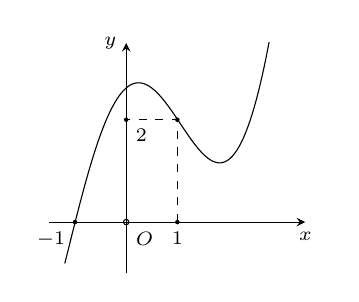
\begin{tikzpicture}[>=stealth,x=1cm,y=1cm,scale=0.65]
		\def\a{-0.04} % Hệ số a phải khác 0
		\def\b{0.26}
		\def\c{0.19}
		\def\d{-1.88}
		\def\e{0.86}
		\def\f{2.62}
		%	\draw[color=gray,dash pattern=on 1pt off 1pt,xstep=1.0cm,ystep=1.0cm] (-5.2,-5.2) grid (5.2,5.2);
		\draw[->] (-1.5,0) -- (3.5,0)node[below]{\scriptsize $x$};
		\draw[->] (0,-1) -- (0,3.5) node[left] {\scriptsize $y$};
		\draw (0,0) circle (1.5pt)node[below right]{\scriptsize $O$};
		\draw[dashed] (1,0)--(1,2)--(0,2);
		\fill (1,0) circle (1.25pt) node[below]{\scriptsize $1$} (-1,0) circle (1.25pt) node[below left]{\scriptsize $-1$} (1,2) circle (1.25pt) (0,2) circle (1.25pt) node[below right]{\scriptsize $2$} ;
		\clip (-1.4,-1)rectangle(4,3.5);
		\draw[samples=150,smooth,domain=-1.2:3.2] plot(\x,{(\a)*(\x)^5+(\b)*(\x)^4+(\c)*(\x)^3+(\d)*(\x)^2+(\e)*(\x)+(\f)});
		\end{tikzpicture}
		
	}
	
	\loigiai{
		\immini
		{Đặt $ t=\sin x-1 $, suy ra $ -2\leq t\leq 0 $.\\
			Phương trình $ f(\sin x-1)=\sin x $, viết lại như sau
			$$f(t)=t+1, \quad t\in [-2;0].$$
			Dựa vào đồ thị hàm số hình bên, suy ra phương trình $ f(t)=t+1 $ có duy nhất nghiệm $ t=-1\in [-2;0] $.\\
			Vậy $ \sin x-1=-1\Leftrightarrow \sin x=0 \Leftrightarrow x=k\pi, \quad k\in \mathbb{Z}$.\\
			Do $ x\in (0;3\pi) $ nên $ 0<k\pi <3\pi $, suy ra $ k\in \{1;2\} $.\\
			Vậy phương trình đã cho có hai nghiệm $ x=\pi $, $ x=2\pi $.	
		}
		{
			% Đồ thị hàm y=ax^3+bx^2+cx+d. Nếu hệ số lớn cần điều chỉnh hệ trục, vùng lưới, domain và lệnh \clip
			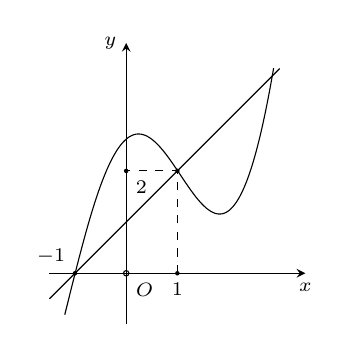
\begin{tikzpicture}[>=stealth,x=1cm,y=1cm,scale=0.65]
			\def\a{-0.04} % Hệ số a phải khác 0
			\def\b{0.26}
			\def\c{0.19}
			\def\d{-1.88}
			\def\e{0.86}
			\def\f{2.62}
			%	\draw[color=gray,dash pattern=on 1pt off 1pt,xstep=1.0cm,ystep=1.0cm] (-5.2,-5.2) grid (5.2,5.2);
			\draw[->] (-1.5,0) -- (3.5,0)node[below]{\scriptsize $x$};
			\draw[->] (0,-1) -- (0,4.5) node[left] {\scriptsize $y$};
			\draw (0,0) circle (1.5pt)node[below right]{\scriptsize $O$};
			\draw[dashed] (1,0)--(1,2)--(0,2);
			\draw (-1.5,-0.5)--(-1,0)--(1,2)--(3,4);
			\fill (1,0) circle (1.25pt) node[below]{\scriptsize $1$} (-1,0) circle (1.25pt) node[above left]{\scriptsize $-1$} (1,2) circle (1.25pt) (0,2) circle (1.25pt) node[below right]{\scriptsize $2$};
			\clip (-1.4,-1)rectangle(4,4);
			\draw[samples=150,smooth,domain=-1.2:3.5] plot(\x,{(\a)*(\x)^5+(\b)*(\x)^4+(\c)*(\x)^3+(\d)*(\x)^2+(\e)*(\x)+(\f)});
			\end{tikzpicture}
		}
		
	}
\end{ex}
\begin{ex}%[GHK1, THPT Nguyễn Thái Bình - Quảng Nam, 2020]%[NAT, 12EX3]%[2H1B3-2]
	Cho khối lăng trụ đứng $ ABC.A'B'C' $ có đáy là tam giác vuông tại $ A $ với $ AB=a $, $ AC=2a\sqrt{3} $, cạnh bên $ AA'=2a $. Thể tích khối lăng trụ $ ABC.A'B'C' $ là
	\choice
	{$a^3$}
	{\True $2\sqrt{3}a^3$}
	{$\sqrt{3}a^3$}
	{$\dfrac{2\sqrt{3}a^3}{3}$}
	\loigiai{
		\immini
		{
			Diện tích đáy $ ABC $ là $ S_{ABC}=\dfrac{1}{2}AB\cdot AC=\sqrt{3}a^2 $.\\
			Thể tích khối lăng trụ $ ABC.A'B'C' $ là $$ V=AA'\cdot S_{ABC}=2a\cdot \sqrt{3}a^2=2\sqrt{3}a^3 .$$
			
		}
		{
			\begin{tikzpicture}[line join=round,line cap=round,line width=.6pt,font=\footnotesize,scale=0.7]
			\coordinate[label=left:$A$] (A) at (0,0);
			\coordinate[label=below left:$B$] (B) at (1,-1);
			\coordinate[label=right:$C$] (C) at (4,0);
			\coordinate[label=left:$A'$] (A1) at ($(A)+(90:4)$);
			\coordinate[label=below left:$B'$] (B1) at ($(B)-(A)+(A1)$);
			\coordinate[label=right:$C'$] (C1) at ($(C)-(A)+(A1)$);
			\draw (A1)--(A)--(B)--(C)--(C1)--(A1)--(B1)--(C1) (B)--(B1);
			\draw[dashed] (A)--(C);
			\tkzMarkRightAngles[size=0.3,fill=gray!50](C,A,B)
			\fill (A)circle(1.5pt) (B)circle(1.5pt) (C)circle(1.5pt) (A1)circle(1.5pt) (B1)circle(1.5pt) (C1)circle(1.5pt);
			\end{tikzpicture}
		}	
		
	}
\end{ex}
\begin{ex}%[GHK1, THPT Nguyễn Thái Bình - Quảng Nam, 2020]%[NAT, 12EX3]%[2H1Y3-2]
	Cho khối chóp có diện tích đáy $ B=3 $ và chiều cao $ h=8 $. Thể tích của khối chóp đã cho bằng
	\choice
	{$6$}
	{$24$}
	{\True $8$}
	{$12$}
	\loigiai{
		Thể tích khối chóp là $ V=\dfrac{1}{3}\cdot 3\cdot 8=8 $.	
		
	}
\end{ex}
\begin{ex}%[GHK1, THPT Nguyễn Thái Bình - Quảng Nam, 2020]%[NAT, 12EX3]%[2D1Y5-3]
	\immini
	{Cho hàm số $ y=ax^4+bx^2+c \ (a, b, c \in \mathbb{R}) $. Đồ thị hàm số $ y=f(x) $ như hình vẽ bên. Số nghệm thực của phương trình $ 2f(x)-3=0 $ là
		\choice
		{$2$}
		{\True $4$}
		{$3$}
		{$0$}}
	{
		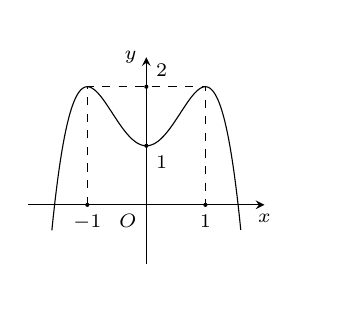
\begin{tikzpicture}[>=stealth,x=1cm,y=1cm,scale=0.75]
		\def\a{-1} % Hệ số a phải khác 0
		\def\b{2}
		\def\c{1}
		\draw[->] (-2,0) -- (2,0)node[below]{\scriptsize $x$};
		\draw[->] (0,-1) -- (0,2.5) node[left] {\scriptsize $y$};
		\fill (-1,0) circle (1pt) node[below]{\scriptsize $-1$} (1,0) circle (1pt) node[below]{\scriptsize $1$} (0,2) circle (1pt) node[above right]{\scriptsize $2$} (0,1) circle (1pt) node[below right]{\scriptsize $1$};
		\draw[dashed] (-1,0)--(-1,2)--(1,2)--(1,0);
		\draw (0,0)node[below left]{\scriptsize $O$};
		\clip (-2,-1.5)rectangle(3,3);
		\draw[samples=150,smooth,domain=-1.6:1.6] plot(\x,{(\a)*(\x)^4+(\b)*(\x)^2+(\c)});
		\end{tikzpicture}
	}
	\loigiai{
		Phương trình $ 2f(x)-3=0\Leftrightarrow f(x)=\dfrac{3}{2} $. Dựa vào đồ thị, suy ra phương trình đã cho có bốn nghiệm phân biệt.
		
	}
\end{ex}
\begin{ex}%[GHK1, THPT Nguyễn Thái Bình - Quảng Nam, 2020]%[NAT, 12EX3]%[2D1Y5-1]
	\immini
	{
		Đồ thị của hàm số nào dưới đây có dạng như đường cong trong hình bên?
		\choice
		{$y=x^4-2x^2$}
		{$y=-x^4+2x^2$}
		{\True $y=-x^3+2x^2$}
		{$y=x^3-3x^2$}
	}
	{
		\begin{tikzpicture}[>=stealth,x=1cm,y=1cm,scale=0.75]
		\def\a{-1} % Hệ số a phải khác 0
		\def\b{2}
		\draw[->] (-1.1,0) -- (3,0)node[below]{\scriptsize $x$};
		\draw[->] (0,-1) -- (0,3) node[left] {\scriptsize $y$};
		\draw [fill=black](0,0)node[below left]{\scriptsize $O$} circle(1pt);
		\clip (-3,-1.5)rectangle(3,3);
		\draw[samples=150,smooth,domain=-1:2.2] plot(\x,{(\a)*(\x)^3+(\b)*(\x)^2});
		\end{tikzpicture}
	}
	
	\loigiai{
		Dựa vào đồ thị hàm số, suy ra, hàm số có dạng $ y=ax^3+bx^2+cx+d $ với $ a<0 $. Hàm số cần tìm là $ y=-x^3+2x^2 $.	
		
	}
\end{ex}
\begin{ex}%[GHK1, THPT Nguyễn Thái Bình - Quảng Nam, 2020]%[NAT, 12EX3]%[2D1B4-1]
	\immini
	{
		Cho hàm số $ y=f(x) $ có bảng biến thiên như hình bên. Tổng số tiệm cận đứng và tiệm cận ngang của đồ thị hàm số là
		\choice
		{\True $2$}
		{$4$}
		{$1$}
		{$3$}
	}
	{
		
\begin{tikzpicture}[>=stealth]
		\tkzTabInit[nocadre=false,lgt=1.2,espcl=2,deltacl=0.5]{$x$/.7 ,$y'$/.7,$y$/2}
		{$-\infty$ , $0$ , $ 1 $, $+\infty$}
		\tkzTabLine{ , -, d , - , z,+, }
		\tkzTabVar{+/$2$ ,-D+/$-4$/$+\infty$ , -/$-2$, +/$ +\infty $}
		\end{tikzpicture}
		
	}
	
	\loigiai{
		Từ bảng biến thiên, suy ra
		\begin{itemize}
			\item $ \lim \limits_{x\to -\infty} y=2 $. Đồ thị hàm số có đường tiệm cận ngang $ y=2 $.
			\item $ \lim \limits_{x\to 0^+} y=+\infty $. Đồ thị hàm số có đường tiệm cận đứng $ x=0 $.
		\end{itemize}	
		Vậy tổng số đường tiệm cận đứng và tiệm cận ngang là $ 2 $. 
	}
\end{ex}
\begin{ex}%[GHK1, THPT Nguyễn Thái Bình - Quảng Nam, 2020]%[NAT, 12EX3]%[2D1B3-1]
	Cho hàm số $ y=\dfrac{x+m}{x-1} $ ($ m $ là tham số thực) thỏa mãn $ \min\limits_{[2;4]} y =3$. Mệnh đề nào dưới đây đúng?
	\choice
	{$m<-1$}
	{$1\leq m<3$}
	{$3<m\leq 4$}
	{\True $m>4$}
	\loigiai{
		Hàm số $ y=\dfrac{x+m}{x-1} $ liên tục trên đoạn $ [2;4] $ và có đạo hàm $ y'=\dfrac{-1-m}{(x-1)^2}, \forall x\in  (2;4)$.\\
		Nếu $m=-1$ thì $y=1$ (loại).\\
		Do đó, hàm số luôn đồng biến hoặc nghịch biến trên $(2;4)$.\\
		Ta có $ y(2)=m+2 $ và $ y(4)=\dfrac{m+4}{3} $.\\
		Trường hợp 1: $ \heva{& y(2)=3 \\ & y(4)\geq y(2)} \Leftrightarrow \heva{& m+2=3 \\ & \dfrac{m+4}{3}\geq m+2.}$	\\
		Hệ này vô nghiệm. Trường hợp này không có giá trị $ m $ thỏa mãn.\\
		Trường hợp 2: $ \heva{& y(4)=3 \\ & y(2)\geq y(4)} \Leftrightarrow \heva{& \dfrac{m+4}{3}=3 \\ & \dfrac{m+4}{3}\leq m+2}\Leftrightarrow m=5.$	\\
		Trường hợp này  $ m=5 $ thỏa mãn.	
	}
\end{ex}
\begin{ex}%[GHK1, THPT Nguyễn Thái Bình - Quảng Nam, 2020]%[NAT, 12EX3]%[2D1Y1-2]
	\immini
	{
		Cho hàm số $ y=f(x) $ có bảng biến thiên như hình bên. Hàm số đã cho đồng biến trên khoảng nào dưới đây?
		\choice
		{$(0;1)$}
		{$(-1;1)$}
		{$(-\infty;-1)$}
		{\True $(-1;0)$}
	}
	{
		% Cần khai báo \usepackage{tkz-tab}
		
\begin{tikzpicture}[>=stealth]
		\tkzTabInit[nocadre=false,lgt=1,espcl=1.5,deltacl=0.5]{$x$/.7 ,$y'$/.7,$y$/2}
		{$-\infty$ , $-1$ ,$ 0 $ ,$1$ , $+\infty$}
		\tkzTabLine{ , - , $0$ , +,$ 0 $, - , $0$ , + , }
		\tkzTabVar{+/$+\infty$ , -/$-1$ , +/$4$ ,-/$ -1 $ , +/$+\infty$}
		\end{tikzpicture}
		
	}
	
	\loigiai{
		Dựa vào bảng biến thiên, suy ra hàm số đồng biến trên khoảng $ (-1;0) $.	
		
	}
\end{ex}
\begin{ex}%[GHK1, THPT Nguyễn Thái Bình - Quảng Nam, 2020]%[NAT, 12EX3]%[2D1B1-2]
	Cho hàm số $ y=f(x) $ liên tục trên $ \mathbb{R} $ và có đạo hàm $ f'(x)=x^2(x+1)^3(x-2), \forall x\in \mathbb{R} $. Hàm số đã cho đồng biến trên khoảng nào dưới đây?
	\choice
	{$(-1;2)$}
	{\True $(-\infty;-1)$}
	{$(-\infty;0)$}
	{$(-1;0)$}
	\loigiai{
		Lập bảng xét dấu của $ f'(x) $, ta có
		\begin{center}
			% Cần khai báo \usepackage{tkz-tab}
			
\begin{tikzpicture}
			\tkzTabInit[nocadre=false,lgt=1.2,espcl=2,deltacl=0.5]{$x$/1 ,$f(x)$/1}
			{$-\infty$ , $-1$ , $0$ , $2$ , $+\infty$}
			\tkzTabLine{ ,+ , 0 , - , 0 , -, 0 , + }
			\end{tikzpicture}
			
		\end{center}
		Dựa vào bảng xét dấu, suy ra hàm số đồng biến trên khoảng $ (-\infty;-1) $.
	}
\end{ex}
\begin{ex}%[GHK1, THPT Nguyễn Thái Bình - Quảng Nam, 2020]%[NAT, 12EX3]%[2H1K3-2]
	Cho hình chóp $ S.ABCD $ có đáy $ ABCD $ là hình thang vuông tại $ A $, $ D $ và $ AB=AD=2a $, $ CD=a $. Góc giữa hai mặt phẳng $ (SBC) $ và $ (ABCD) $ bằng $ 60^\circ $. Gọi $ I $ là trung điểm của $ AD $, biết hai mặt phẳng $ (SBI) $, $ (SCI) $ cùng vuông góc với mặt phẳng $ (ABCD) $. Tính thể tích của khối chóp $ S.ABCD $.
	\choice
	{\True $\dfrac{3\sqrt{15}a^3}{5}$}
	{$\dfrac{3\sqrt{23}a^3}{5}$}
	{$\dfrac{3\sqrt{19}a^3}{5}$}
	{$\dfrac{3\sqrt{17}a^3}{5}$}
	\loigiai{
		\immini
		{
			Vì $ SI=(SBI)\cap (SCI) $ và $ (SBI) $, $ (SCI) $ cùng vuông góc với đáy nên $ SI\perp (ABCD) $.\\
			Xét tam giác $ IBC $, có $ IC=a\sqrt{2} $, $ IB=a\sqrt{5}$.\\
			Và $ BC=a\sqrt{5} $.\\
			Gọi $ F $ là đỉnh thứ ba của hình vuông $ ABFD $, gọi $ H=IF\cap BC $, suy ra $ IF\perp BC $.\\
			Suy ra $ \widehat{SHI}=60^\circ $. Xét tam giác $ BFC $, có
			$$BH\cdot BC=BF^2\Rightarrow \dfrac{BH}{BC}	=\dfrac{BF^2}{BC^2}=\dfrac{4}{5}.$$
			Hay $ BH=\dfrac{4}{5}\cdot \sqrt{5}a=\dfrac{4a}{\sqrt{5}} $.\\ Từ đó, suy ra
			$ IH=\sqrt{IB^2-BH^2}=\dfrac{3a}{\sqrt{5}} $.
		}
		{
			\begin{tikzpicture}[line join=round,line cap=round,line width=.6pt,font=\footnotesize,scale=1]
			\coordinate[label=below left:$D$] (D) at (0,-2);
			\coordinate[label=above right:$A$] (A) at (1,1);
			\coordinate[label=below right:$C$] (C) at (3,-2);
			\coordinate[label=above right:$B$] (B) at (7,1);
			\coordinate[label=left:$I$] (I) at ($(A)!.5!(D)$);
			%	\coordinate[label=above:$E$] (E) at ($(A)!.5!(B)$);
			\coordinate[label=right:$F$] (F) at ($(D)+(B)-(A)$);
			\coordinate[label=left:$S$] (S) at ($(I)+(90:4)$);
			\coordinate[label=above:$H$] (H) at ($(B)!4/5!(C)$);
			\tkzMarkRightAngles[size=0.2,fill=gray!50](S,I,B I,H,C)
			\draw (D)--(C)--(B)--(S)--cycle (S)--(C) (C)--(F)--(B) (F)--(H)--(S);
			\draw[dashed] (I)--(C)--(A)--(B)--(I)--(S)--(A)--(D)--(B) (I)--(H);
			\fill (A)circle(1.5pt) (B)circle(1.5pt) (C)circle(1.5pt) (D)circle(1.5pt) (S)circle(1.5pt) (I)circle(1.5pt)  (F)circle(1.5pt) (H)circle(1.5pt);
			\end{tikzpicture}
			
		}	
		\noindent Xét tam giác $ SIH $ vuông tại $ I $, có $ SI=IH\cdot \tan 60^\circ=\dfrac{3\sqrt{3}a}{\sqrt{5}} $. Thể tích khối chóp là
		$$V=\dfrac{1}{3}\cdot \dfrac{3\sqrt{3}a}{\sqrt{5}} \cdot 3a^2=\dfrac{3\sqrt{15}a^3}{5}.$$	
	}
\end{ex}
\begin{ex}%[GHK1, THPT Nguyễn Thái Bình - Quảng Nam, 2020]%[NAT, 12EX3]%[2D1B5-3]
	Tìm tất cả các giá trị thực của tham số $ m $ để phương trình $ -x^4+2x^2=m-3 $ có bốn nghiệm thực phân biệt.
	\choice
	{$0<m<1$}
	{$3\leq m \leq 4$}
	{$m>3$}
	{\True $ 3<m<4$}
	\loigiai{
		Phương trình đã cho viết lại $ -x^4+2x^2+3=m $.\\
		Đặt $ f(x)=-x^4+2x^2+3 $, lập bảng biến thiên của hàm số $ f(x) $ ta được
		\begin{center}
			% Cần khai báo \usepackage{tkz-tab}
			
\begin{tikzpicture}[>=stealth]
			\tkzTabInit[nocadre=false,lgt=1.2,espcl=2.5,deltacl=0.5]{$x$/.7 ,$y'$/.7,$y$/2}
			{$-\infty$ , $-1$ ,$ 0 $, $1$ , $+\infty$}
			\tkzTabLine{ , + , $0$ , -,$0$ ,+ , $0$ , - , }
			\tkzTabVar{-/$-\infty$ ,+/$ 4 $ ,-/$3$ , +/$4$ , -/$-\infty$}
			\end{tikzpicture}
			
		\end{center}	
		Dựa vào bảng biến thiên, phương trình đã cho có bốn nghiệm thực phân biệt khi và chỉ khi $ m\in (3;4) $.	
	}
\end{ex}
\begin{ex}%[GHK1, THPT Nguyễn Thái Bình - Quảng Nam, 2020]%[NAT, 12EX3]%[2H1B2-3]
	Số mặt đối xứng của hình lập phương là 
	\choice
	{\True $9$}
	{$7$}
	{$6$}
	{$5$}
	\loigiai{
		Số mặt đối xứng của hình lập phương là $ 9 $.
		\begin{center}
			\begin{tikzpicture}[scale=0.7, font=\footnotesize, line join=round, line cap=round, >=stealth]
			\tkzDefPoints{0/0/A,-2/-1/B,1/-1/C}
			\coordinate (D) at ($(A)+(C)-(B)$);
			\coordinate (A') at ($(A)+(0,2.5)$);
			\tkzDefPointsBy[translation=from A to A'](B,C,D){B'}{C'}{D'}
			\tkzDrawPolygon[draw = white, fill= gray, opacity=.2](A,C,C',A')
			\tkzDrawPolygon(A',B',B,C,D,D')
			\tkzDrawSegments(B',C' C',D' C,C')
			\tkzDrawSegments[dashed](A,B A,D A,A')
			\end{tikzpicture} $\quad$ $\quad$
			\begin{tikzpicture}[scale=0.7, font=\footnotesize, line join=round, line cap=round, >=stealth]
			\tkzDefPoints{0/0/A,-2/-1/B,1/-1/C}
			\coordinate (D) at ($(A)+(C)-(B)$);
			\coordinate (A') at ($(A)+(0,2.5)$);
			\tkzDefPointsBy[translation=from A to A'](B,C,D){B'}{C'}{D'}
			\tkzDrawPolygon[draw = white, fill= gray, opacity=.2](B,D,D',B')
			\tkzDrawPolygon(A',B',B,C,D,D')
			\tkzDrawSegments(B',C' C',D' C,C')
			\tkzDrawSegments[dashed](A,B A,D A,A')
			\end{tikzpicture} $\quad$ $\quad$
			\begin{tikzpicture}[scale=0.7, font=\footnotesize, line join=round, line cap=round, >=stealth]
			\tkzDefPoints{0/0/A,-2/-1/B,1/-1/C}
			\coordinate (D) at ($(A)+(C)-(B)$);
			\coordinate (A') at ($(A)+(0,2.5)$);
			\tkzDefPointsBy[translation=from A to A'](B,C,D){B'}{C'}{D'}
			\coordinate (M) at ($(C)!1/2!(B)$);
			\coordinate (N) at ($(C')!1/2!(B')$);
			\coordinate (P) at ($(A)!1/2!(D)$);
			\coordinate (Q) at ($(A')!1/2!(D')$);
			\tkzDrawPolygon[draw = white, fill= gray, opacity=.2](M,N,Q,P)
			\tkzDrawPolygon(A',B',B,C,D,D')
			\tkzDrawSegments(B',C' C',D' C,C')
			\tkzDrawSegments[dashed](A,B A,D A,A')
			\end{tikzpicture}\\
			\begin{tikzpicture}[scale=0.7, font=\footnotesize, line join=round, line cap=round, >=stealth]
			\tkzDefPoints{0/0/A,-2/-1/B,1/-1/C}
			\coordinate (D) at ($(A)+(C)-(B)$);
			\coordinate (A') at ($(A)+(0,2.5)$);
			\tkzDefPointsBy[translation=from A to A'](B,C,D){B'}{C'}{D'}
			\coordinate (M) at ($(A)!1/2!(B)$);
			\coordinate (N) at ($(A')!1/2!(B')$);
			\coordinate (P) at ($(C)!1/2!(D)$);
			\coordinate (Q) at ($(C')!1/2!(D')$);
			\tkzDrawPolygon[draw = white, fill= gray, opacity=.2](M,N,Q,P)
			\tkzDrawPolygon(A',B',B,C,D,D')
			\tkzDrawSegments(B',C' C',D' C,C')
			\tkzDrawSegments[dashed](A,B A,D A,A')
			\end{tikzpicture} $\quad$ $\quad$
			\begin{tikzpicture}[scale=0.7, font=\footnotesize, line join=round, line cap=round, >=stealth]
			\tkzDefPoints{0/0/A,-2/-1/B,1/-1/C}
			\coordinate (D) at ($(A)+(C)-(B)$);
			\coordinate (A') at ($(A)+(0,2.5)$);
			\tkzDefPointsBy[translation=from A to A'](B,C,D){B'}{C'}{D'}
			\coordinate (M) at ($(A)!1/2!(A')$);
			\coordinate (N) at ($(B)!1/2!(B')$);
			\coordinate (P) at ($(C)!1/2!(C')$);
			\coordinate (Q) at ($(D)!1/2!(D')$);
			\tkzDrawPolygon[draw = white, fill= gray, opacity=.2](M,N,P,Q)
			\tkzDrawPolygon(A',B',B,C,D,D')
			\tkzDrawSegments(B',C' C',D' C,C')
			\tkzDrawSegments[dashed](A,B A,D A,A')
			\end{tikzpicture} $\quad$ $\quad$
			\begin{tikzpicture}[scale=0.7, font=\footnotesize, line join=round, line cap=round, >=stealth]
			\tkzDefPoints{0/0/A,-2/-1/B,1/-1/C}
			\coordinate (D) at ($(A)+(C)-(B)$);
			\coordinate (A') at ($(A)+(0,2.5)$);
			\tkzDefPointsBy[translation=from A to A'](B,C,D){B'}{C'}{D'}
			\tkzDrawPolygon[draw = white, fill= gray, opacity=.2](A',D',C,B)
			\tkzDrawPolygon(A',B',B,C,D,D')
			\tkzDrawSegments(B',C' C',D' C,C')
			\tkzDrawSegments[dashed](A,B A,D A,A')
			\end{tikzpicture} \\
			\begin{tikzpicture}[scale=0.7, font=\footnotesize, line join=round, line cap=round, >=stealth]
			\tkzDefPoints{0/0/A,-2/-1/B,1/-1/C}
			\coordinate (D) at ($(A)+(C)-(B)$);
			\coordinate (A') at ($(A)+(0,2.5)$);
			\tkzDefPointsBy[translation=from A to A'](B,C,D){B'}{C'}{D'}
			\tkzDrawPolygon[draw = white, fill= gray, opacity=.2](A,D,C',B')
			\tkzDrawPolygon(A',B',B,C,D,D')
			\tkzDrawSegments(B',C' C',D' C,C')
			\tkzDrawSegments[dashed](A,B A,D A,A')
			\end{tikzpicture} $\quad$ $\quad$
			\begin{tikzpicture}[scale=0.7, font=\footnotesize, line join=round, line cap=round, >=stealth]
			\tkzDefPoints{0/0/A,-2/-1/B,1/-1/C}
			\coordinate (D) at ($(A)+(C)-(B)$);
			\coordinate (A') at ($(A)+(0,2.5)$);
			\tkzDefPointsBy[translation=from A to A'](B,C,D){B'}{C'}{D'}
			\tkzDrawPolygon[draw = white, fill= gray, opacity=.2](A',B',C,D)
			\tkzDrawPolygon(A',B',B,C,D,D')
			\tkzDrawSegments(B',C' C',D' C,C')
			\tkzDrawSegments[dashed](A,B A,D A,A')
			\end{tikzpicture} $\quad$ $\quad$
			\begin{tikzpicture}[scale=0.7, font=\footnotesize, line join=round, line cap=round, >=stealth]
			\tkzDefPoints{0/0/A,-2/-1/B,1/-1/C}
			\coordinate (D) at ($(A)+(C)-(B)$);
			\coordinate (A') at ($(A)+(0,2.5)$);
			\tkzDefPointsBy[translation=from A to A'](B,C,D){B'}{C'}{D'}
			\tkzDrawPolygon[draw = white, fill= gray, opacity=.2](A,B,C',D')
			\tkzDrawPolygon(A',B',B,C,D,D')
			\tkzDrawSegments(B',C' C',D' C,C')
			\tkzDrawSegments[dashed](A,B A,D A,A')
			\end{tikzpicture} 
		\end{center}			
		
	}
\end{ex}
\begin{ex}%[GHK1, THPT Nguyễn Thái Bình - Quảng Nam, 2020]%[NAT, 12EX3]%[2D1K1-3]
	Tổng $ S $ tất cả các giá trị nguyên của tham số $ m $ để hàm số $ y=\dfrac{x+3}{x-m} $ nghịch biến trên khoảng $ (2020;+\infty) $ là
	\choice
	{\True $S=2041207$}
	{$S=2041204$}
	{$S=4082408$}
	{$S=4082414$}
	\loigiai{
		Tập xác định của hàm số là $ \mathscr{D}=(-\infty;m)\cup (m;+\infty) $.\\
		Đạo hàm $ y'=\dfrac{-m-3}{(x-m)^2} $ với $ x\in \mathscr{D} $.\\
		Yêu cầu bài toán trở thành
		$$\heva{& -m-3<0 \\ & m\notin (2020;+\infty)}\Leftrightarrow \heva{& m>-3 \\ & m\leq 2020}\Leftrightarrow -3<m\leq 2020.$$	
		Do $ m\in \mathbb{Z} $ nên $ m\in \{-2;-1;0;1;2;3;4;5;6;\ldots;2020\} $. Tổng các giá trị $ m $ nguyên thỏa mãn yêu cầu bài toán là
		$$S=(-2)+(-1)+0+1+2+3+4+5+6+\cdots+2020=2041207.$$
	}
\end{ex}
\begin{ex}%[GHK1, THPT Nguyễn Thái Bình - Quảng Nam, 2020]%[NAT, 12EX3]%[2D1Y2-1]
	Giá trị cực tiểu của hàm số $ y=x^4-4x^2-2 $ là
	\choice
	{$-2$}
	{\True $-6$}
	{$-8$}
	{$10$}
	\loigiai{
		Lập bảng biến thiên của hàm số 	$ y=x^4-4x^2-2 $, ta có
		\begin{center}
			% Cần khai báo \usepackage{tkz-tab}
			
\begin{tikzpicture}[>=stealth]
			\tkzTabInit[nocadre=false,lgt=1.2,espcl=2.5,deltacl=0.5]{$x$/.7 ,$y'$/.7,$y$/2}
			{$-\infty$ , $-\sqrt{2}$ ,$ 0 $, $\sqrt{2}$ , $+\infty$}
			\tkzTabLine{ , - , $0$ , +,$0$ ,- , $0$ , + , }
			\tkzTabVar{+/$+\infty$ ,-/$ -6 $ ,+/$-2$ , -/$-6$ , +/$+\infty$}
			\end{tikzpicture}
			
		\end{center}	
		Từ bảng biến thiên, suy ra 	giá trị cực tiểu của hàm số $ y=x^4-4x^2-2 $ là $ -6 $.
	}
\end{ex}
\begin{ex}%[GHK1, THPT Nguyễn Thái Bình - Quảng Nam, 2020]%[NAT, 12EX3]%[2D1Y5-1]
	\immini
	{Đồ thị của hàm số nào dưới đây có dạng như đường cong hình bên?
		\choice
		{\True $y=x^4-2x^2$}
		{$y=-x^3+3x^2$}
		{$y=-x^4+2x^2$}
		{$y=x^3-3x^2$}
	}
	{
		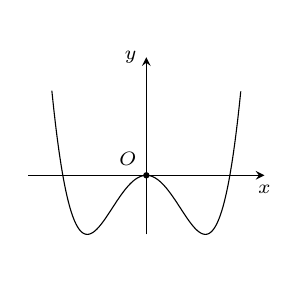
\begin{tikzpicture}[>=stealth,x=1cm,y=1cm,scale=0.75]
		\def\a{1} % Hệ số a phải khác 0
		\def\b{-2}
		\draw[->] (-2,0) -- (2,0)node[below]{\scriptsize $x$};
		\draw[->] (0,-1) -- (0,2) node[left] {\scriptsize $y$};
		\draw[fill=black] (0,0) circle(1.25pt)node[above left]{\scriptsize $O$};
		\clip (-2,-1.5)rectangle(2,2.5);
		\draw[samples=150,smooth,domain=-1.6:1.6] plot(\x,{(\a)*(\x)^4+(\b)*(\x)^2});
		\end{tikzpicture}
	}
	
	\loigiai{
		Đồ thị hàm số có ba điểm cực trị, hàm số có dạng $ y=ax^4+bx^2+c $ với $ a>0 $. Hàm số cần tìm là $y=x^4-2x^2$.	
		
	}
\end{ex}
\begin{ex}%[GHK1, THPT Nguyễn Thái Bình - Quảng Nam, 2020]%[NAT, 12EX3]%[2H1B3-2]
	Cho hình chóp $S.ABCD$ có đáy $ ABCD $ là hình vuông cạnh $ a $, $ SA\perp (ABCD) $. Cạnh bên $ SC $ tạo với đáy một góc $ 45^\circ $. Thể tích của khối chóp $ S.ABCD $ là
	\choice
	{$\sqrt{2}a^3$}
	{$\dfrac{a^3}{3}$}
	{$\dfrac{\sqrt{3}a^3}{3}$}
	{\True $\dfrac{\sqrt{2}a^3}{3}$}
	\loigiai{
		\immini
		{
			Diện tích đáy $ ABCD $ là $ S_{ABCD}=a^2 $.\\
			Xét tam giác $ SAC $ có $ \widehat{SAC}=45^\circ $ và vuông tại $ A $ nên $ SA=AC=a\sqrt{2} $.\\
			Vậy thể tích khối chóp $ S.ABCD $ là $$ V_{S.ABCD}=\dfrac{1}{3}\cdot SA\cdot S_{ABCD}=\dfrac{1}{3}\cdot a\sqrt{2}\cdot a^2=\dfrac{\sqrt{2}a^3}{3}. $$
		}
		{
			\begin{tikzpicture}[line join=round,line cap=round,line width=.6pt,font=\footnotesize,scale=1]
			\coordinate[label=below left:$B$] (B) at (0,0);
			\coordinate[label=above left:$A$] (A) at (1,.8);
			\coordinate[label=below right:$C$] (C) at (4,0);
			\coordinate[label=above right:$D$] (D) at ($(C)-(B)+(A)$);
			\coordinate[label=above left:$S$] (S) at ($(A)+(90:3)$);
			\draw (B)--(C)--(D)--(S)--cycle (S)--(C);
			\draw[dashed] (C)--(A)--(D) (S)--(A)--(B);
			\draw ($ (A)!5pt!(D)$)--($(A)!2!($($(A)!5pt!(D)$)!.5!($(A)!5pt!(S)$)$)$)--($(A)!5pt!(S)$);
			\fill (A)circle(1.5pt) (B)circle(1.5pt) (C)circle(1.5pt) (D)circle(1.5pt) (S)circle(1.5pt);
			\end{tikzpicture}
			
		}
		
	}
\end{ex}
\begin{ex}%[GHK1, THPT Nguyễn Thái Bình - Quảng Nam, 2020]%[NAT, 12EX3]%[2H1K3-2]
	Cho hình chóp $S.ABCD$ có đáy $ ABCD $ là hình chữ nhật, tam giác $ SAB $ đều và nằm trong mặt phẳng vuông góc với đáy, $ AB=a $, mặt bên $ (SCD) $ tạo với đáy một góc bằng $ 30^\circ $. Thể tích của khối chóp $ S.ABCD $ là
	\choice
	{$a^3\sqrt{3}$}
	{\True $\dfrac{\sqrt{3}a^3}{4}$}
	{$\dfrac{\sqrt{3}a^3}{12}$}
	{$\dfrac{3\sqrt{3}a^3}{4}$}
	\loigiai{
		\immini
		{
			Gọi $ H $ là trung điểm $ AB $, suy ra $ AH\perp (ABCD) $.\\
			Gọi $ K $ là trung điểm $ CD $, suy ra tam giác $ SHK $ vuông tại $ H $ và $ \widehat{SKH}=30^\circ $.\\
			Tam giác $ SAB $ đều cạnh $ a $, suy ra $ SH=\dfrac{a\sqrt{3}}{2} $.\\
			Xét tam giác $ SHK $ vuông tại $ H $, có $ \widehat{SKH}=30^\circ $ nên $ HK=SH\cdot \cot 30^\circ= \dfrac{a\sqrt{3}}{2}\cdot \sqrt{3}=\dfrac{3a}{2}$.\\
			Vậy, diện tích đáy $ ABCD $ là $$ S_{ABCD}=AB\cdot BC=a\cdot \dfrac{3a}{2}=\dfrac{3a^2}{2}. $$
		}
		{
			\begin{tikzpicture}[line join=round,line cap=round,line width=.6pt,font=\footnotesize,scale=1]
			\coordinate[label=below left:$B$] (B) at (0,0);
			\coordinate[label=above left:$A$] (A) at (1.5,.8);
			\coordinate[label=below right:$C$] (C) at (4,0);
			\coordinate[label=above right:$D$] (D) at ($(C)-(B)+(A)$);
			\coordinate[label=above left:$H$] (H) at ($(A)!1/2!(B)$); % Thay đổi số 1/2 để đổi vị trí điểm H
			\coordinate[label=below right:$K$] (K) at ($(C)!1/2!(D)$); 
			\coordinate[label=above left:$S$] (S) at ($(H)+(90:4)$);
			\draw (B)--(C)--(D)--(S)--cycle (S)--(C) (S)--(K);
			\draw[dashed] (A)--(D) (K)--(H)--(S)--(A)--(B);
			\draw ($ (H)!5pt!(A)$)--($(H)!2!($($(H)!5pt!(A)$)!.5!($(H)!5pt!(S)$)$)$)--($(H)!5pt!(S)$);
			\fill (A)circle(1.5pt) (B)circle(1.5pt) (C)circle(1.5pt) (D)circle(1.5pt) (S)circle(1.5pt) (H)circle(1.5pt) (K)circle(1.5pt);
			\end{tikzpicture}
			
		}
		\noindent	Thể tích khối chóp $ S.ABCD $ là
		$V=\dfrac{1}{3}\cdot SH\cdot S_{ABCD}=\dfrac{1}{3}\cdot \dfrac{a\sqrt{3}}{2}\cdot \dfrac{3a^2}{2}=\dfrac{\sqrt{3}a^3}{4}$.
	}
\end{ex}

\Closesolutionfile{ans}
\begin{indapan}{10}
	{ans/ans-2-GHK1-32-NguyenThaiBinh-QuangNam-21}
\end{indapan}
